\documentclass[a4paper,12pt]{article}

\usepackage[utf8]{inputenc}
\usepackage[english]{babel}
\usepackage{natbib}
\usepackage[T1]{fontenc}
\usepackage{setspace}
\usepackage{graphicx}
\usepackage{hyperref}

\graphicspath{ {images/} }

\title{\vspace{2cm}\textbf{Design Statement}}
\author{Joshua Bridge\\14032908\\joshua.m.bridge@stu.mmu.ac.uk}

\begin{document}

\maketitle

\tableofcontents

\listoffigures

\doublespacing

\newpage

\section{Requirements}
  The application proposed in this report would be best utilised on multiple platforms \& devices, as the service it would offer is platform-independent (i.e. all you need is an image file). For this reason the primary focus will be making an online web-app, which connects to a seperate REST \citep{fielding2000architectural} API which performs the main functions of the application, without the clutter of the front-end mixing in with it. This would also allow other apps and services to utilise this API and integrate it with other apps, such as on social media apps when sharing an image.

  When designing a user-facing website and an API, there are certain considerations that have to be met, such as data security and ease of use. The following features define what the final product should achieve:

  \begin{itemize}
    \item A web-based user interface.
    \item A user-history (metadata) tracking mechanism.
    \item A RESTful API which can be utilised by any application.
  \end{itemize}

  Following these features, these are some of the things that should be taken into consideration when implementing these features:

    \begin{itemize}
      \item The application \& API should be able to handle a high-volume amount of users.
      \item It should not store any more information about users than it has to.
      \item It should make this data available at a users request.
      \item It should maintain a reasonable level of security to prevent user-data from being stolen.
      \item It should not store any user images after the user has finished using the application.
    \end{itemize}

\section{Technologies}

  \subsection{Front-end}

    \subsubsection{Angular JS}

  \subsection{Back-end (Python)}

    \subsubsection{Django}

  \subsection{API (Python)}

    \subsubsection{Flask}

    % \subsubsection{Celery}

  \subsection{Deployment - AWS}

    \begin{figure}[ht]
      \centering
      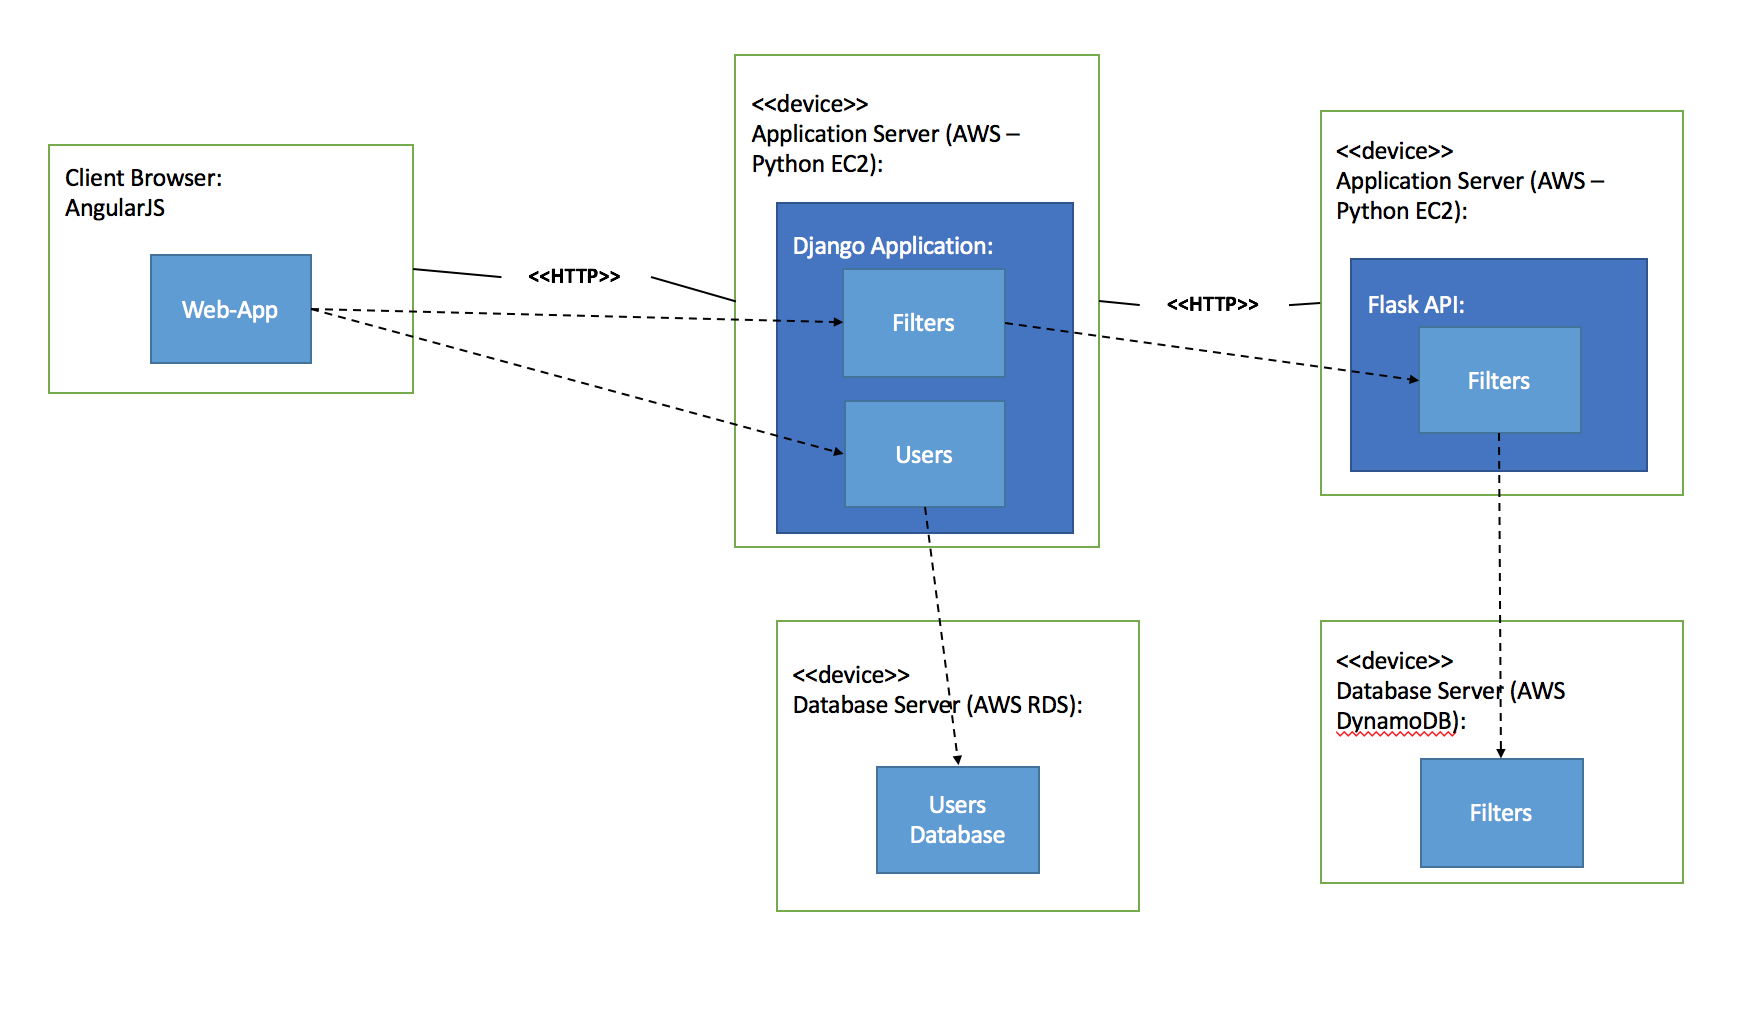
\includegraphics[width=\linewidth]{deployment-diagram}
      \caption{Component deployment diagram}
      \label{fig:deployment-diagram}
    \end{figure}

    Fig. \ref{fig:deployment-diagram} defines the component layout for the entire workflow of the application proposed in this report.

% \section{Data structures}


\newpage
\singlespacing

\bibliographystyle{agsm}
\bibliography{design}


\end{document}
